\section*{Results of Verification through modal calculus formulas}
In order to check the formulae the lbs2pbes and pbes2Bool tool has been used. In addition to the global requirements, the system was checked and is verified to be \underline{deadlock free} through the formula  \textbf{[true*] $<$true$>$ true}. The results from the verification of the global requirements are presented in the following table.

The verification results for all the global requirements are listed below. \ref{tab: verification}.

\begin{table}[h]
\centering
\begin{tabular}{|l|l|l|}\hline
Requirement & Result \\\hline
1.1 & true  \\\hline
1.2 & true \\\hline
1.3.1 & true \\\hline
1.3.2 & true \\\hline
1.4 & true \\\hline
2 &  true \\\hline
3 &  true \\\hline
4.1 &  true \\\hline
4.2 &  true \\\hline
5 &  true \\\hline
6 &  true \\\hline
7 &  true \\\hline
8 &  Not verified\\\hline
9 &  true \\\hline

\end{tabular}
\caption{Verification results}
\label{tab: verification}
\end{table}

\subsection*{Verification through trace scenarios}
In order to verify the behaviour of the system, in addition to the fulfillment of the global requirements, we have simulated the following scenarios by using the ``xsim`` from the LPS tool.

The figure \ref{fig:xsim1} below shows the usage of the simulation of the LPS.

\begin{figure}[h]
\center
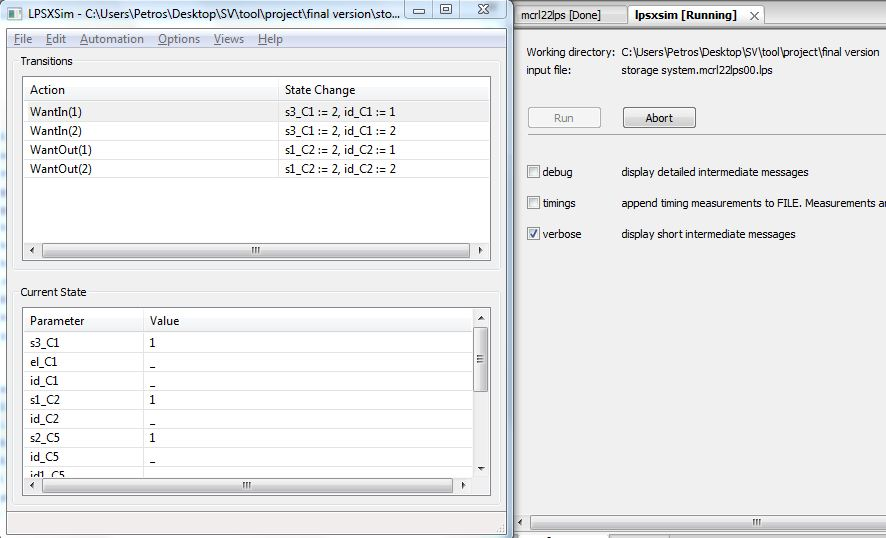
\includegraphics[width=0.8\textwidth]{xsim}
\caption{Simulation of the LPS with xsim}
\label{fig:xsim1}
\end{figure}

\begin{itemize}
\item
In this scenario, we have simulated the case that, initially a packet with “id” is inserted to the system and then another packet with same “id” is tried to be inserted into the system. The simulation results in a case that the second package is rejected \textbf{(CheckSameID.trc)}.

\item  This “.trc” files simulates the case where, the packet is inserted to the system and then it is requested and removed. Moreover, it has been tried to request the packet which is already removed from the system. Naturally, this request resulted in PacketNotFound action which should be considered as expected behavior of the system\\ \textbf{(Ins\_Pckt\_Req\_Pckt\_TryToReqSamePckt\_Again.trc)}.

\item In this scenario, the case that, the packets are delivered in the same order, is simulated. Initially, two packets are inserted to the system and then packets with id ``1`` and ``2`` are requested consecutively. It can be seen that the packets are delivered in the same order \textbf{(sameorder.trc)}.
\end{itemize}

\section*{Verification through LTS}
In this part, LTS graph for the different requirements are presented. Since, the diagrams of complicated requirements produce significantly large number of states (more than 30 states), only the understandable diagrams are included in this report. In order to obtain abstract LTS diagrams, we hide all the actions which are irrelevant for the requirement that is supposed to be examined. The ltsconvert tool is used by specifying parameter as tau-star.  In order to reduce the number of states in the LTS graph, “MaxPacketID” is determined as ''1''. Note that ''maxPacketID'' refers to number of different ''id'' that system will produce.

\begin{figure}[h]
\center
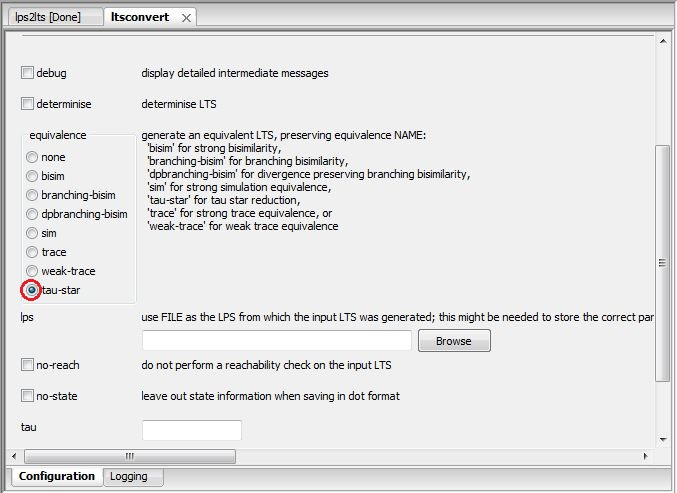
\includegraphics[width=0.8\textwidth]{ltsconvert}
\caption{LtsConvert}
\label{fig:ltsconvert}
\end{figure}

\begin{enumerate}

\item
Requirement 2:  Packet is exchanged only when the elevator platform is at the same level as that of a conveyor belt. (Figure \ref{fig:req2})

\begin{figure}[h]
\center
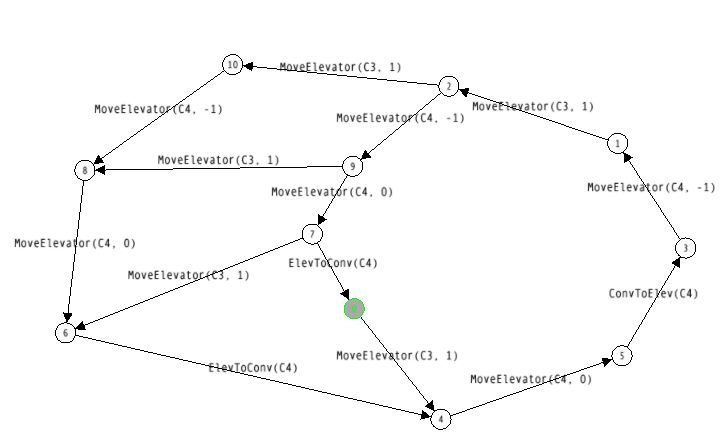
\includegraphics[width=0.8\textwidth]{req2}
\caption{Requirement 2 verification}
\label{fig:req2}
\end{figure}

In order to present the LTS with smaller number of states, all the actions other than ``MoveElevator``, ``ConvToElev`` and ``ElevToConv`` are hidden. As it was already mentioned previously in this report, the packets can be exchanged between the elevators and the conveyor belts (ConvIn and ConvOut) only in position ``0``. It is possible to observe from figure above that, C3 is moved to position ``1`` before ``MoveElevator(C4,0)`` action takes place. By considering these consecutive actions, it is possible to state that, the two elevators cannot be at same position (state 9).


\item Requirement 3: Packet is exchanged only when the elevator platform is at the same level as that of the rack.

\begin{figure}[h]
\center
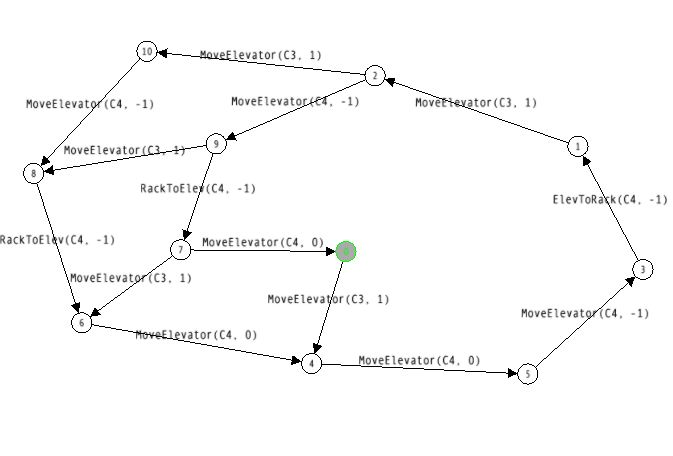
\includegraphics[width=0.8\textwidth]{req3}
\caption{Requirement 3 verification}
\label{fig:req3}
\end{figure}

The LTS graph which can be seen in figure \ref{fig:req2} is obtained by hiding all the actions other than ``MoveElevator``, ``RackToElev`` and ``ElevToRack``. In order to understand that the corresponding requirement is fulfilled or not, last MoveElevator action before RackToElev or ElevToRack is found  in the LTS graph. By using this approach, we can guarantee that the transfer of the packet is performed to the expected position successfully. The scenario that is explained in the previous sentence regarding the behavior of the RackToElev action can be observed in the following states ``10``, ``8``, ``6``, ``2``, ``9`` and ``7`` as well. Moreover, the similar behaviour for ElevToRack can be seen in states ``5``, ``3`` and ``1``. As it was mentioned before, Since the LTS graphs are obtained by using only ``1`` id, the system can accept one packet which will be transported to ``-1`` position by ``C4`` elevator.

\item Requirement 5: The lower elevator must never pass the upper one.

\begin{figure}[h]
\center
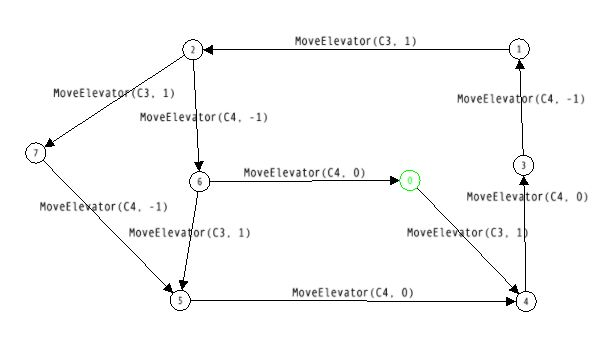
\includegraphics[width=0.8\textwidth]{req5}
\caption{Requirement 5 verification}
\label{fig:req5}
\end{figure}

In order to present the LTS all the actions except MoveElevator are hidden. This is seen in figure \ref{fig:req5} In order to specify that this requirement is verified, there should not be any path which includes MoveElevator(C3, x) action and MoveElevator(C4, y) with y > x. One may find the situation that is explained by tracking the states from the initial state. Having two or more than two ``id`` would make the state space too large to have included in this report; limiting this requirement to a single ``id``  can still be adequately described.


\end{enumerate}

\section*{Conclusions}
In this project, we learnt to work with the mCRL2 code, verification tools and analysing complex LTS graphs and ways to interpret it in simpler ways using the tool. In the end, the efforts were fruitful. All but one requirement was verified for the designed model. The requirement that could not be fulfilled was due to not verifying the property satisfactorily due to the limitation stated in the translated requirements.